% Options for packages loaded elsewhere
\PassOptionsToPackage{unicode}{hyperref}
\PassOptionsToPackage{hyphens}{url}
%
\documentclass[
]{article}
\usepackage{lmodern}
\usepackage{amssymb,amsmath}
\usepackage{ifxetex,ifluatex}
\ifnum 0\ifxetex 1\fi\ifluatex 1\fi=0 % if pdftex
  \usepackage[T1]{fontenc}
  \usepackage[utf8]{inputenc}
  \usepackage{textcomp} % provide euro and other symbols
\else % if luatex or xetex
  \usepackage{unicode-math}
  \defaultfontfeatures{Scale=MatchLowercase}
  \defaultfontfeatures[\rmfamily]{Ligatures=TeX,Scale=1}
\fi
% Use upquote if available, for straight quotes in verbatim environments
\IfFileExists{upquote.sty}{\usepackage{upquote}}{}
\IfFileExists{microtype.sty}{% use microtype if available
  \usepackage[]{microtype}
  \UseMicrotypeSet[protrusion]{basicmath} % disable protrusion for tt fonts
}{}
\makeatletter
\@ifundefined{KOMAClassName}{% if non-KOMA class
  \IfFileExists{parskip.sty}{%
    \usepackage{parskip}
  }{% else
    \setlength{\parindent}{0pt}
    \setlength{\parskip}{6pt plus 2pt minus 1pt}}
}{% if KOMA class
  \KOMAoptions{parskip=half}}
\makeatother
\usepackage{xcolor}
\IfFileExists{xurl.sty}{\usepackage{xurl}}{} % add URL line breaks if available
\IfFileExists{bookmark.sty}{\usepackage{bookmark}}{\usepackage{hyperref}}
\hypersetup{
  pdftitle={Heart Disease},
  pdfauthor={Andrea Cantarutti},
  hidelinks,
  pdfcreator={LaTeX via pandoc}}
\urlstyle{same} % disable monospaced font for URLs
\usepackage[margin=1in]{geometry}
\usepackage{color}
\usepackage{fancyvrb}
\newcommand{\VerbBar}{|}
\newcommand{\VERB}{\Verb[commandchars=\\\{\}]}
\DefineVerbatimEnvironment{Highlighting}{Verbatim}{commandchars=\\\{\}}
% Add ',fontsize=\small' for more characters per line
\usepackage{framed}
\definecolor{shadecolor}{RGB}{248,248,248}
\newenvironment{Shaded}{\begin{snugshade}}{\end{snugshade}}
\newcommand{\AlertTok}[1]{\textcolor[rgb]{0.94,0.16,0.16}{#1}}
\newcommand{\AnnotationTok}[1]{\textcolor[rgb]{0.56,0.35,0.01}{\textbf{\textit{#1}}}}
\newcommand{\AttributeTok}[1]{\textcolor[rgb]{0.77,0.63,0.00}{#1}}
\newcommand{\BaseNTok}[1]{\textcolor[rgb]{0.00,0.00,0.81}{#1}}
\newcommand{\BuiltInTok}[1]{#1}
\newcommand{\CharTok}[1]{\textcolor[rgb]{0.31,0.60,0.02}{#1}}
\newcommand{\CommentTok}[1]{\textcolor[rgb]{0.56,0.35,0.01}{\textit{#1}}}
\newcommand{\CommentVarTok}[1]{\textcolor[rgb]{0.56,0.35,0.01}{\textbf{\textit{#1}}}}
\newcommand{\ConstantTok}[1]{\textcolor[rgb]{0.00,0.00,0.00}{#1}}
\newcommand{\ControlFlowTok}[1]{\textcolor[rgb]{0.13,0.29,0.53}{\textbf{#1}}}
\newcommand{\DataTypeTok}[1]{\textcolor[rgb]{0.13,0.29,0.53}{#1}}
\newcommand{\DecValTok}[1]{\textcolor[rgb]{0.00,0.00,0.81}{#1}}
\newcommand{\DocumentationTok}[1]{\textcolor[rgb]{0.56,0.35,0.01}{\textbf{\textit{#1}}}}
\newcommand{\ErrorTok}[1]{\textcolor[rgb]{0.64,0.00,0.00}{\textbf{#1}}}
\newcommand{\ExtensionTok}[1]{#1}
\newcommand{\FloatTok}[1]{\textcolor[rgb]{0.00,0.00,0.81}{#1}}
\newcommand{\FunctionTok}[1]{\textcolor[rgb]{0.00,0.00,0.00}{#1}}
\newcommand{\ImportTok}[1]{#1}
\newcommand{\InformationTok}[1]{\textcolor[rgb]{0.56,0.35,0.01}{\textbf{\textit{#1}}}}
\newcommand{\KeywordTok}[1]{\textcolor[rgb]{0.13,0.29,0.53}{\textbf{#1}}}
\newcommand{\NormalTok}[1]{#1}
\newcommand{\OperatorTok}[1]{\textcolor[rgb]{0.81,0.36,0.00}{\textbf{#1}}}
\newcommand{\OtherTok}[1]{\textcolor[rgb]{0.56,0.35,0.01}{#1}}
\newcommand{\PreprocessorTok}[1]{\textcolor[rgb]{0.56,0.35,0.01}{\textit{#1}}}
\newcommand{\RegionMarkerTok}[1]{#1}
\newcommand{\SpecialCharTok}[1]{\textcolor[rgb]{0.00,0.00,0.00}{#1}}
\newcommand{\SpecialStringTok}[1]{\textcolor[rgb]{0.31,0.60,0.02}{#1}}
\newcommand{\StringTok}[1]{\textcolor[rgb]{0.31,0.60,0.02}{#1}}
\newcommand{\VariableTok}[1]{\textcolor[rgb]{0.00,0.00,0.00}{#1}}
\newcommand{\VerbatimStringTok}[1]{\textcolor[rgb]{0.31,0.60,0.02}{#1}}
\newcommand{\WarningTok}[1]{\textcolor[rgb]{0.56,0.35,0.01}{\textbf{\textit{#1}}}}
\usepackage{graphicx,grffile}
\makeatletter
\def\maxwidth{\ifdim\Gin@nat@width>\linewidth\linewidth\else\Gin@nat@width\fi}
\def\maxheight{\ifdim\Gin@nat@height>\textheight\textheight\else\Gin@nat@height\fi}
\makeatother
% Scale images if necessary, so that they will not overflow the page
% margins by default, and it is still possible to overwrite the defaults
% using explicit options in \includegraphics[width, height, ...]{}
\setkeys{Gin}{width=\maxwidth,height=\maxheight,keepaspectratio}
% Set default figure placement to htbp
\makeatletter
\def\fps@figure{htbp}
\makeatother
\setlength{\emergencystretch}{3em} % prevent overfull lines
\providecommand{\tightlist}{%
  \setlength{\itemsep}{0pt}\setlength{\parskip}{0pt}}
\setcounter{secnumdepth}{-\maxdimen} % remove section numbering

\title{Heart Disease}
\author{Andrea Cantarutti}
\date{8/5/2020}

\begin{document}
\maketitle

\hypertarget{what-causes-heart-disease}{%
\subsection{What causes heart
disease?}\label{what-causes-heart-disease}}

Including libraries needed for the analysis purpose

\begin{Shaded}
\begin{Highlighting}[]
\KeywordTok{library}\NormalTok{(ggplot2)}
\KeywordTok{library}\NormalTok{(tidyr)}
\KeywordTok{library}\NormalTok{(tidyverse)}
\KeywordTok{library}\NormalTok{(dplyr)}
\KeywordTok{library}\NormalTok{(readr)}
\end{Highlighting}
\end{Shaded}

Let's import data and tidy them according to the dataset specifications
The variables included are: - Age - Sex - CP (type of chest pain) -
Trestbps (resting blood pressure) - Chol (Serum Cholesterol value, LDL
and HDL together. Should be less than 200) - FBS (Fasting blood sugar
\textgreater{} 120 mg/dl (1 true, 0 false)) - RestECG (Resting
electrocardiographs results (0, 1, 2)) - THLACH (Maximum heart rate
achieved) - EXAng (Exercise induced angina) - Oldpeak (q) - Slope (the
slope of the ST depression) - CA (number of major vessels (0-3) colored
by flourosopy) - Thal: 3 = normal; 6 = fixed defect; 7 = reversable
defect - Target (1: disease, 0: healty)

\begin{Shaded}
\begin{Highlighting}[]
\NormalTok{heart <-}\StringTok{ }\KeywordTok{read.csv}\NormalTok{(}\StringTok{'heart2.csv'}\NormalTok{)}

\KeywordTok{names}\NormalTok{(heart) <-}\StringTok{ }\KeywordTok{c}\NormalTok{(}\StringTok{"Age"}\NormalTok{, }\StringTok{"Sex"}\NormalTok{, }\StringTok{"ChestPain"}\NormalTok{, }\StringTok{"RestingBloodPressure"}\NormalTok{, }\StringTok{"Cholesterol"}\NormalTok{, }\StringTok{"FastingBloogSugar"}\NormalTok{, }\StringTok{"RestECG"}\NormalTok{, }\StringTok{"MaxHeartRate"}\NormalTok{, }\StringTok{"ExerciseAngina"}\NormalTok{, }\StringTok{"OldPeak"}\NormalTok{,}
                  \StringTok{"PeakSlope"}\NormalTok{, }\StringTok{"MajorVessels"}\NormalTok{, }\StringTok{"Thal"}\NormalTok{, }\StringTok{"HasDisease"}\NormalTok{)}

\NormalTok{cases <-}\StringTok{ }\KeywordTok{count}\NormalTok{(heart)}

\NormalTok{heart =}\StringTok{ }\NormalTok{heart }\OperatorTok
\StringTok{  }\KeywordTok{mutate}\NormalTok{(}\DataTypeTok{Sex =} \KeywordTok{case_when}\NormalTok{(Sex }\OperatorTok{==}\StringTok{ }\DecValTok{1} \OperatorTok{~}\StringTok{ "M"}\NormalTok{, Sex }\OperatorTok{==}\StringTok{ }\DecValTok{0} \OperatorTok{~}\StringTok{ "F"}\NormalTok{),}
         \DataTypeTok{FastingBloogSugar =} \KeywordTok{case_when}\NormalTok{(FastingBloogSugar }\OperatorTok{==}\StringTok{ }\DecValTok{1} \OperatorTok{~}\StringTok{ "T"}\NormalTok{, FastingBloogSugar }\OperatorTok{==}\StringTok{ }\DecValTok{0} \OperatorTok{~}\StringTok{ "F"}\NormalTok{),}
         \DataTypeTok{ExerciseAngina =} \KeywordTok{case_when}\NormalTok{(ExerciseAngina }\OperatorTok{==}\StringTok{ }\DecValTok{1} \OperatorTok{~}\StringTok{ "T"}\NormalTok{, ExerciseAngina }\OperatorTok{==}\StringTok{ }\DecValTok{0} \OperatorTok{~}\StringTok{ "F"}\NormalTok{),}
         \DataTypeTok{HasDisease =} \KeywordTok{case_when}\NormalTok{(HasDisease }\OperatorTok{==}\StringTok{ }\DecValTok{1} \OperatorTok{~}\StringTok{ "T"}\NormalTok{, HasDisease }\OperatorTok{==}\StringTok{ }\DecValTok{0} \OperatorTok{~}\StringTok{ "F"}\NormalTok{)}
\NormalTok{  )}
\end{Highlighting}
\end{Shaded}

Let's plot some information just to get the big picture of the whole
dataset and start exploring the data

\begin{Shaded}
\begin{Highlighting}[]
\NormalTok{heart }\OperatorTok\StringTok{ }
\StringTok{  }\KeywordTok{group_by}\NormalTok{(HasDisease) }\OperatorTok\StringTok{ }
\StringTok{  }\KeywordTok{summarise}\NormalTok{(}\DataTypeTok{n =} \KeywordTok{n}\NormalTok{()) }\OperatorTok
\StringTok{  }\KeywordTok{ggplot}\NormalTok{(}\KeywordTok{aes}\NormalTok{(}\DataTypeTok{x =}\NormalTok{ HasDisease, }\DataTypeTok{y =}\NormalTok{ n)) }\OperatorTok{+}
\StringTok{  }\KeywordTok{geom_bar}\NormalTok{(}\DataTypeTok{stat=}\StringTok{"identity"}\NormalTok{, }\DataTypeTok{fill=}\StringTok{"lightblue"}\NormalTok{) }\OperatorTok{+}
\StringTok{  }\KeywordTok{labs}\NormalTok{(}\DataTypeTok{x =} \StringTok{"Has Disease"}\NormalTok{, }\DataTypeTok{y =} \StringTok{"Count"}\NormalTok{) }\OperatorTok{+}\StringTok{ }
\StringTok{  }\KeywordTok{geom_text}\NormalTok{(}\DataTypeTok{stat=}\StringTok{'identity'}\NormalTok{, }\KeywordTok{aes}\NormalTok{(}\DataTypeTok{label=}\NormalTok{n), }\DataTypeTok{vjust=}\DecValTok{10}\NormalTok{, }\DataTypeTok{fontface=}\StringTok{"bold"}\NormalTok{, }\DataTypeTok{size=}\DecValTok{6}\NormalTok{)}
\end{Highlighting}
\end{Shaded}

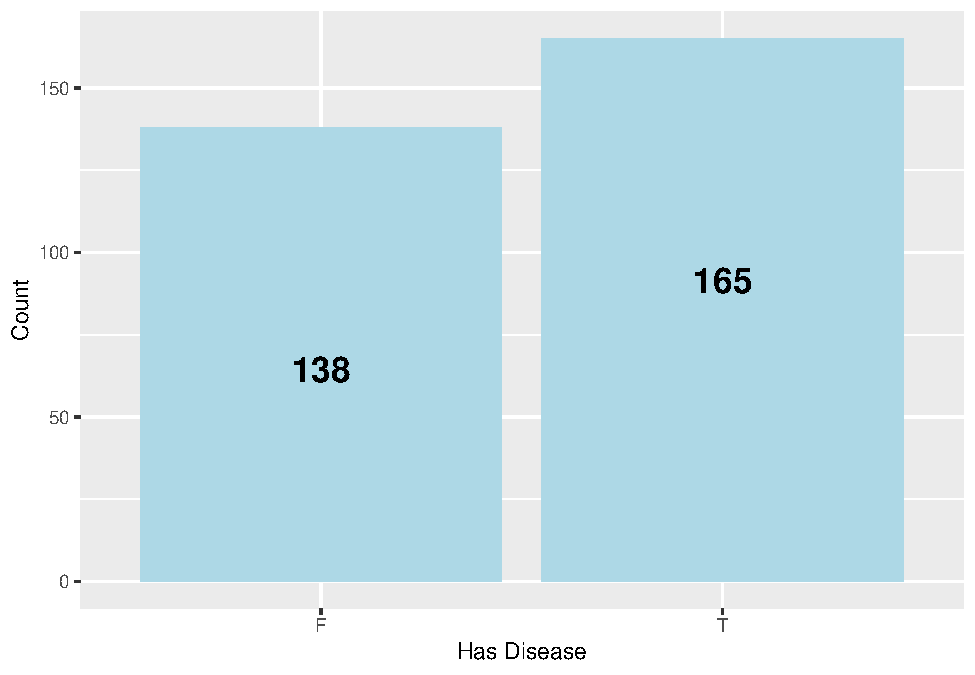
\includegraphics{heart_files/figure-latex/unnamed-chunk-3-1.pdf}

Let's find out what's the distribution of males and females between
people affected or not by heart disease

\begin{Shaded}
\begin{Highlighting}[]
\NormalTok{SexDeasease <-}\StringTok{ }\NormalTok{heart }\OperatorTok
\StringTok{  }\KeywordTok{group_by}\NormalTok{(HasDisease, Sex) }\OperatorTok
\StringTok{  }\KeywordTok{summarise}\NormalTok{(}\DataTypeTok{per=}\KeywordTok{n}\NormalTok{()}\OperatorTok{/}\NormalTok{cases, }\DataTypeTok{absolute_count =} \KeywordTok{n}\NormalTok{()) }\OperatorTok
\StringTok{  }\KeywordTok{mutate}\NormalTok{(}\DataTypeTok{per =} \KeywordTok{round}\NormalTok{(per}\OperatorTok{*}\DecValTok{100}\NormalTok{,}\DecValTok{2}\NormalTok{))}

\NormalTok{labels =}\StringTok{ }\NormalTok{SexDeasease}\OperatorTok{$}\NormalTok{per}\OperatorTok{$}\NormalTok{n}

\KeywordTok{ggplot}\NormalTok{(SexDeasease, }\KeywordTok{aes}\NormalTok{(}\DataTypeTok{x=}\NormalTok{HasDisease, }\DataTypeTok{y=}\NormalTok{absolute_count, }\DataTypeTok{colour=}\NormalTok{Sex)) }\OperatorTok{+}
\StringTok{    }\KeywordTok{geom_bar}\NormalTok{(}\DataTypeTok{stat=}\StringTok{"identity"}\NormalTok{, }\DataTypeTok{fill=}\StringTok{"lightgrey"}\NormalTok{) }\OperatorTok{+}
\StringTok{    }\KeywordTok{labs}\NormalTok{(}\DataTypeTok{x =} \StringTok{"Has Disease"}\NormalTok{, }\DataTypeTok{y =} \StringTok{"Count"}\NormalTok{) }\OperatorTok{+}
\StringTok{    }\CommentTok{# geom_text(aes(label=labels, colour=Sex), vjust=0, fontface="bold", size=4)}
\StringTok{    }\KeywordTok{theme_dark}\NormalTok{()}
\end{Highlighting}
\end{Shaded}

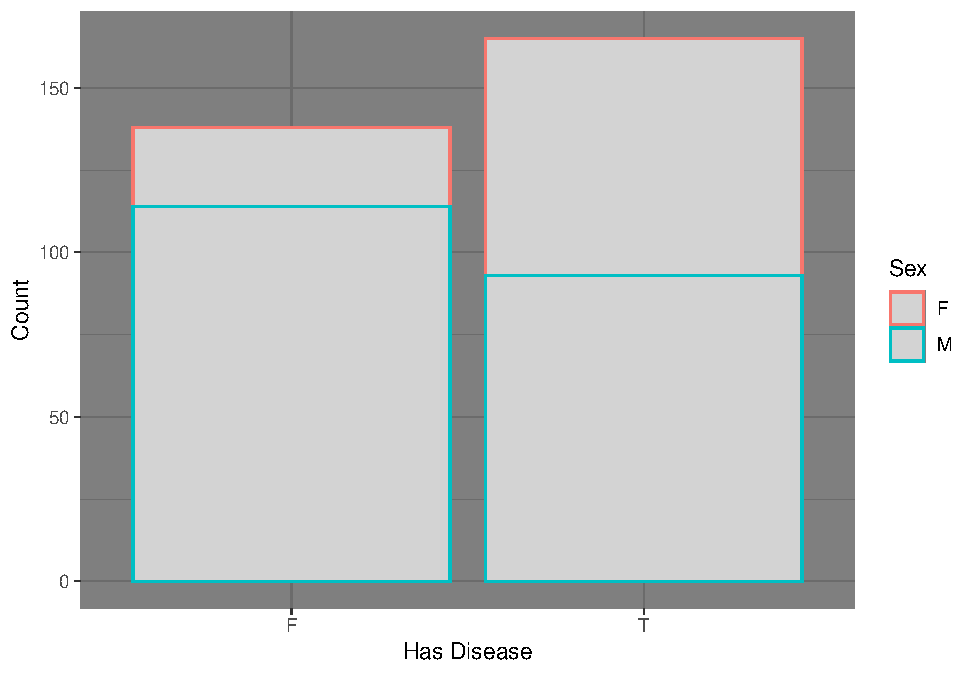
\includegraphics{heart_files/figure-latex/unnamed-chunk-4-1.pdf}

Let's now find out the distribution of male and female people affected
by the disease

\begin{Shaded}
\begin{Highlighting}[]
\KeywordTok{library}\NormalTok{(plotrix)}
\NormalTok{percentage <-}\StringTok{ }\NormalTok{heart }\OperatorTok
\StringTok{  }\KeywordTok{filter}\NormalTok{(HasDisease }\OperatorTok{==}\StringTok{ "T"}\NormalTok{) }\OperatorTok
\StringTok{  }\KeywordTok{group_by}\NormalTok{(Sex) }\OperatorTok
\StringTok{  }\KeywordTok{summarise}\NormalTok{(}\DataTypeTok{per=}\KeywordTok{n}\NormalTok{()}\OperatorTok{/}\NormalTok{cases, }\DataTypeTok{absolute_count =} \KeywordTok{n}\NormalTok{())}

\NormalTok{bc <-}\StringTok{ }\KeywordTok{pie3D}\NormalTok{(percentage}\OperatorTok{$}\NormalTok{per}\OperatorTok{$}\NormalTok{n, }\DataTypeTok{explode=}\DecValTok{0}\NormalTok{, }\DataTypeTok{main=}\StringTok{"Visualization of male and female people affected by heart disease"}\NormalTok{, }\DataTypeTok{theta=}\DecValTok{1}\NormalTok{)}
\KeywordTok{pie3D.labels}\NormalTok{(bc, }\DataTypeTok{labels=}\KeywordTok{c}\NormalTok{(}\StringTok{"Female"}\NormalTok{, }\StringTok{"Male"}\NormalTok{), }\DataTypeTok{radius=}\FloatTok{0.5}\NormalTok{, }\DataTypeTok{labelcex =} \DecValTok{1}\NormalTok{, }\DataTypeTok{theta=}\DecValTok{2}\NormalTok{)}
\end{Highlighting}
\end{Shaded}

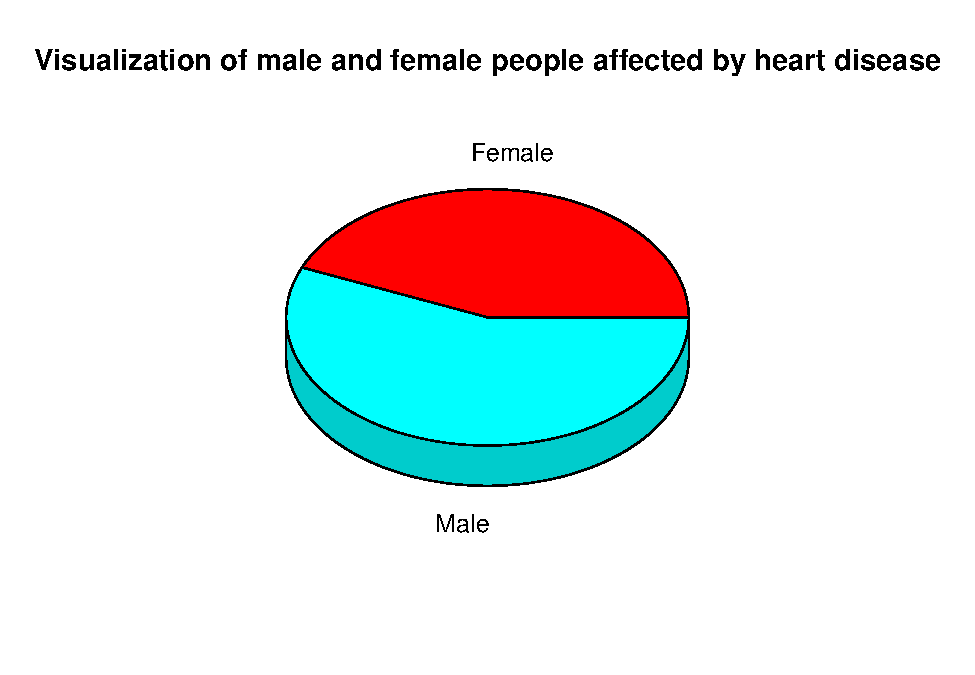
\includegraphics{heart_files/figure-latex/unnamed-chunk-5-1.pdf}

\end{document}
